\documentclass{article}
\usepackage[utf8]{inputenc}
\usepackage{amsmath}
\usepackage{amssymb}
\usepackage{mathtools}
\usepackage{graphicx}

\graphicspath{{Images/}}


\setlength{\oddsidemargin}{0in}
\setlength{\textwidth}{6.5in}
\setlength{\topmargin}{-.55in}
\setlength{\textheight}{9in}
\pagestyle{empty}


\title{Solid State Physics HW1}
\author{Michael Nameika}
\date{September 2022}

\begin{document}

\maketitle

\textbf{1. \textit{Tetrahedral angles.}} The angles between the tetrahedral bonds of diamond are the same as the angles between the body diagonals of a cube, as in Fig. 10. Use elementary vector analysis to find the value of the angle.
\newline\newline


To begin, we will approach this problem by looking at the unit cube and considering the body diagonals from the vertices $(0,0,0)$ to $(1,1,1)$ and from $(1,1,0)$ to $(0,0,1)$. Notice that these body diagonals can be represented by the following vectors in $\mathbb{R}^3$:
\[\textbf{v}_1 = \begin{bmatrix}
    1\\
    1\\
    1\\
\end{bmatrix}\]
and
\[\textbf{v}_2 = \begin{bmatrix*}[r]
    -1\\
    -1\\
    1\\
\end{bmatrix*}\]

The following illustration shows the unit cube with the vectors $\textbf{v}_1$ and $\textbf{v}_2$ (the red and blue lines, respectively):

\begin{center}
    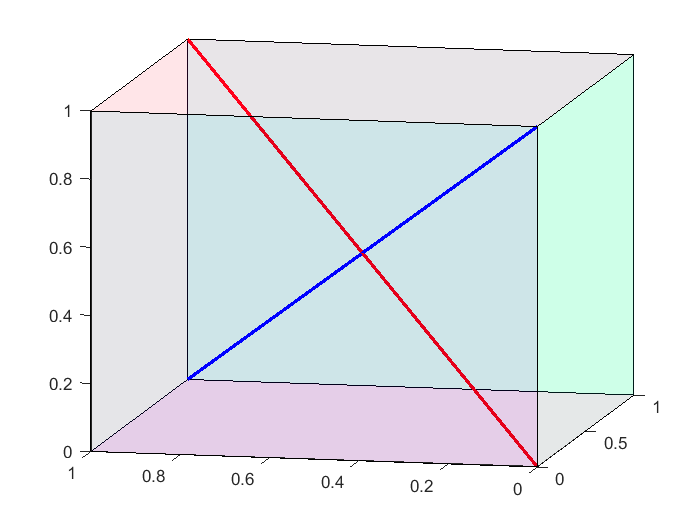
\includegraphics[scale = 0.6]{UNITCUBE.png}
\end{center}

Recall the formula that relates the angle between two vectors to their inner product:
\begin{equation}
    \textbf{v}_1 \cdot \textbf{v}_2 = ||\textbf{v}_1||||\textbf{v}_2||\cos{(\theta)}
\end{equation}

Where $|| \cdot ||$ denotes the Euclidean norm. Taking the inner product of $\textbf{v}_1$ and $\textbf{v}_2$, we find
\[\textbf{v}_1 \cdot \textbf{v}_2 = -1 + -1 + 1 = -1\]
and the magnitudes of $\textbf{v}_1$ and $\textbf{v}_2$ are given by
\[||\textbf{v}_1|| = ||\textbf{v}_2|| = \sqrt{3}\]
Then solving equation (1) for $\theta$, we find
\[\theta = \arccos\left(-{\frac{1}{3}}\right)\]
\[\approx 109.5^{\circ}\]
That is, the body diagonals of a cube intersect at an angle of approximately $109.5^{\circ}$.
\newline\newline

\textbf{2. \textit{Indices of planes.}} Consider the planes with indices $(100)$ and $(001)$; the lattice is fcc, and the indices refer to the conventional cubic cell. What are the indices of these planes when referred to the primitive axes of Fig.11?
\newline\newline
\begin{center}
    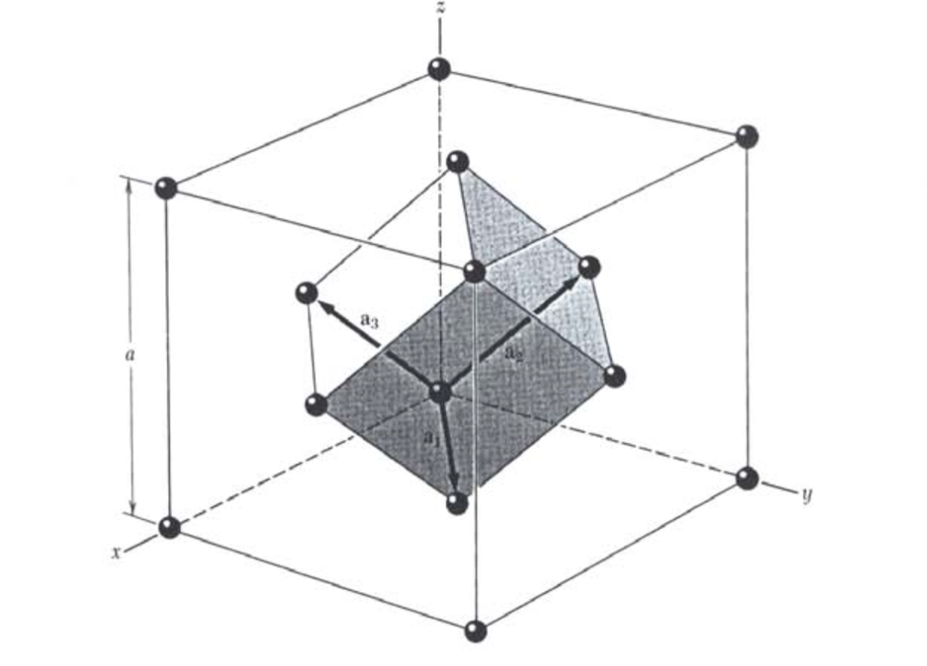
\includegraphics[scale = 0.6]{cubefigure.PNG}
\end{center}


We wish to find the Miller indices for the $(100)$ plane for the primitive axes given by $\textbf{a}_1$, $\textbf{a}_2$, and $\textbf{a}_3$. Notice that the $(100)$ plane will cut the primitive axes at $(2,+\infty,2)$. Then to find the Miller index for this plane, we must take the reciprocal of the elements and normalize to the smallest integer. Well, the reciprocals give us $\left(\frac{1}{2}, 0 , \frac{1}{2}\right)$. Normalizing to the smallest integer, we get $(101)$ as the Miller index for the primitive axes. 
\newline


Now we wish to find the Miller indices for the primitive axes for the plane $(001)$ in the conventional cubic cell. Similar to the $(100)$ plane, the $(001)$ plane will intersect the primitive axes at the point $(+\infty,2,2)$. From similar logic above, the Miller index in the primitive axes will be
$(011)$.
\newline\newline

\textbf{3. \textit{Hcp structure.}} Show that the $c/a$ ratio for an ideal hexagonal close-packed structure is $\left(\frac{8}{3}\right)^{1/2} \approx 1.633$. If $c/a$ is significantly larger than this value, the crystal structure may be thought of as composed of planes of closely packed atoms, the planes being loosely stacked.
\newline\newline

We wish to find the ratio $c/a$ for an ideal hexagonal close-packed structure. Recall that there are two atoms per unit cell in the close-packed hexagonal structure (hcp) and that the volume of the unit cell is given by
\[V = \frac{\sqrt{3}}{2}a^2c\]

Let $PE$ denote the packing efficiency, $N$ the number of atoms per unit cell, and $v_s$ the volume of the 'atomic sphere'. Quickly note that the nearest neighbor distance in the hcp structure is $a$. Then the radius of the atomic sphere is $a/2$. Recall that there are $2$ atoms per unit cell in the hcp structure and since the atomic sphere's radius is $a/2$,
\[v_s = \frac{4\pi}{3}\left(\frac{a}{2}\right)^3\]
Now, recall that the formula for packing efficiency is given by
\begin{equation}
    PE = \frac{Nv_s}{V}
\end{equation}
Plugging in what we have for $V$, $N$, and $v_s$ into (2), we find
\[PE = \frac{2 \cdot \frac{4\pi}{3}\cdot \frac{a^3}{8}}{\frac{\sqrt{3}}{2}a^2c}\]
Simplifying, we get

\begin{equation}
    PE = \frac{8\pi a}{3\sqrt{3}c}
\end{equation}

Additionally, recall that the ideal stacking efficiency is given by
\[PE_{\text{ideal}} = \frac{\pi}{3\sqrt{2}}\]
Setting (3) equal to $PE_{\text{ideal}}$, we get
\[\frac{8\pi a}{3 \sqrt{3}c} = \frac{\pi}{3\sqrt{2}}\]
Simplifying and solving for $c/a$, we get
\[\frac{c}{a} = \left(\frac{8}{3}\right)^{1/2}\]
Which is what we wished to show.
\begin{flushright}
    $\square$
\end{flushright}

\end{document}
